\documentclass{cnriut} % Ne pas modifier
\annee{2025}           % Ne pas modifier
\lieu{Bayonne} % Ne pas modifier

\usepackage{graphicx}  % inclusion de graphiques
\usepackage{biblatex}
\addbibresource{references.bib}
\usepackage{tabularx}

\titre{Développement d'un framework de suivi et d'évaluation de l'impact à travers un data warehouse semantique pour les meta-organisations}

% \auteurs{%
%   Clément Combier$^{1,*}$ \and
%   Adel Noureddine$^2$ \and
%   Jose Enrique Armendariz-Inigo$^3$ \and
%   Philippe Arnould $^2$
%   }

% \courriels{%
%   clement.combier@univ-pau.fr \and
%   adel.noureddine@univ-pau.fr    \and
%   enrique.armendariz@unavarra.es \and
%   philippe.arnould@univ-pau.fr
% }


\affiliations{%
  $^1$ Université de Pau et des Pays de l'Adour \\
   E2S-UPPA, LIUPPA, Mont de Marsan, France \\
  \\
  $^2$ IUT de Pays de l'Adour \\
  E2S-UPPA, LIUPPA, Mont de Marsan, France\\
  \\
   $^3$ Universidad Pública de Navarra \\
  Pampelune, Espagne\\
}

\correspondingauthors{Le/les auteur(s) avec la marque * sont auteur(s) correspondant(s).}

\themes{%
 Gestion - Informatique - Communication 
}

\resume{Ce travail de recherche vise à développer un cadre pour les méta-organisations (notamment les alliances d'universités européennes) pour surveiller et évaluer leur impact sur la société en utilisant des solutions données. Les alliances d'universités européennes, telles que celles créées dans le cadre de l'initiative européenne des universités, nécessitent des outils et des méthodologies spécifiques pour évaluer leur impact, qui dépasse celui des organisations individuelles. Ce cadre devra prendre en compte la complexité des organisations interconnectées et la nécessité de flexibilité pour répondre aux besoins spécifiques de chaque organisation membre.}

\motscles{data warehouse, web semantic, meta-organisation}

\sectionsCNU{27}

%CONSERVER LA VALEUR "OUI" OU "NON" si l'article sera présenté par un doctorant durant le CNRIUT'2025.
\doctorant{OUI}


\begin{document}
\creationEnTete        % Ne pas modifier

\section{Introduction}
La globalisation et l'internationalisation de l'éducation ont connu une accélération spectaculaire ces dernières années, en particulier au sein des établissements d'enseignement supérieur. Ce mouvement mondial s'est popularisé en Europe grâce à l'initiative Erasmus+ des universités européennes. En 2019, l'initiative des universités européennes (EUI) a été lancée avec pour mission de promouvoir, de faciliter et de diffuser la nécessité d'alliances interuniversitaires en Europe. Depuis, 64 alliances, couvrant plus de 35 pays, regroupant plus de 500 universités ont été créées. Ces alliances entraînent des changements et des transformations importantes, apportant de nouveaux besoins et défis. Pour assurer le développement et la durabilité des universités européennes à venir, il est nécessaire de surveiller et d'évaluer l'impact lié à la vision à long terme de ces alliances.

Les alliances européennes pourraient être caractérisées en suivant le modèle proposé en 2005 par G Ahrne et N Brunsson \cite{ahrne_organizations_2005}, en appliquant le concept de meta-organisation pour désigner le regroupement de nombreuses organisations autour d'objectifs et projets commun. 

De nombreux frameworks et méthodologies ont été développés et proposés au fil des ans sur la théorie des changements et  d'évaluation de l'impact. Cependant, ces cadres peuvent ne pas fournir aux meta-organisations les outils et la flexibilité des organisations simples. Ceci prouve l'importance d'une méthodologie plus large pour les meta-organisations, tout en gardant une ancre pour chaque organisation partenaire.

Ce projet de recherche vise à développer un cadre pour les meta-organisations (dans ce contexte, les alliances d'universités européennes) pour surveiller et évaluer leur impact sur la société en utilisant des solutions orientées données.

\section{État de l'art}
Ce rapport d'état de l'art fournira une introduction du paysage de la recherche sur la mesure de l'impact, la théorie du changement, les systèmes de suivi et d'évaluation dans le contexte des meta-organisations. En s'appuyant dans notre cas sur les alliances d'universités. 

Alors que nous nous concentrons sur différents axes autour de notre cadre potentiel, nous avons étudié notre problématique à travers différents prismes et angles. 
Commençons par définir l'impact et la méthodologie utilisée. Nous allons utiliser la définition suivante du Comité d'aide au développement (CAD) de l'Organisation de coopération et de développement économiques (OCDE) :

« Effets à long terme, positifs et négatifs, directs et indirects, intentionnels et non intentionnels produits par une intervention de développement »\cite{oecd_quality_2010}

\begin{figure}
    \centering
    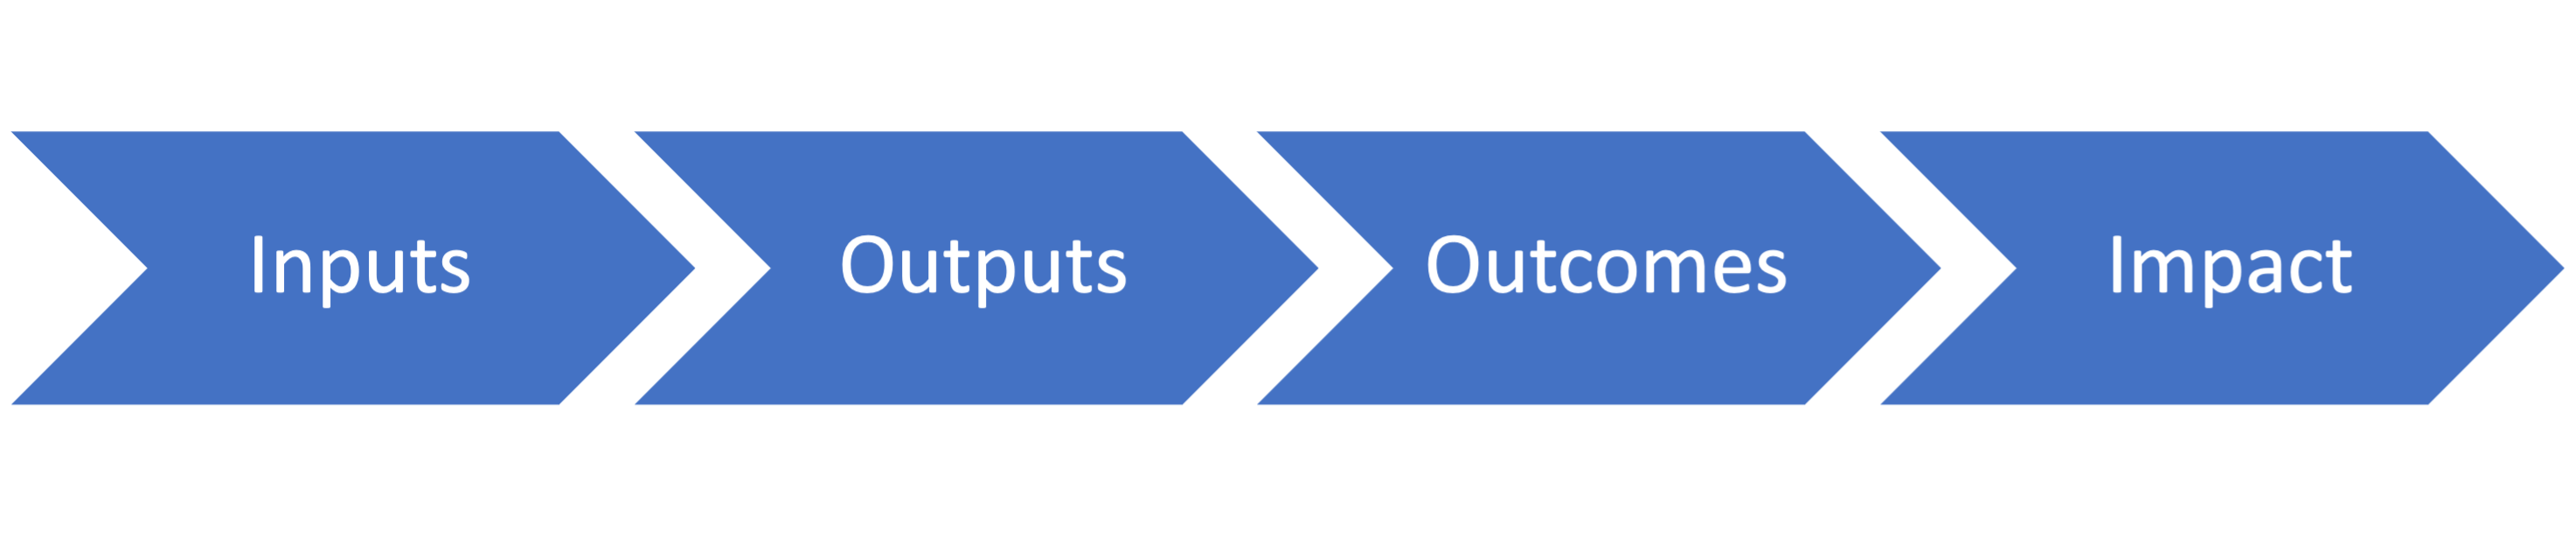
\includegraphics[width=1\linewidth]{Modele_Latex_CNRIUT2025//images/impact-chain.png}
    \caption{Chaîne de mesure d’impac\cite{stein_understanding_2012}}
    \label{fig:impact-chain}
\end{figure}
Maintenant, en s'appuyant sur la figure \ref{fig:impact-chain}, nous allons définir ses termes.
\begin{itemize}
    \item Inputs: Représentent les ressources et les matériaux nécessaires pour lancer un projet ou un programme.
    \item Outputs: Résultats directs et immédiats des activités, souvent quantifiables et mesurables.
    \item Outcomes: Indiquent les réalisations initiales résultant des sorties et des activités, contribuant aux objectifs du projet.
    \item Impact: Représente les effets à long terme et les changements plus larges qui se produisent en raison du projet, influençant les parties prenantes et la communauté.
\end{itemize}

Étant donné que le point suivant a été largement accepté et reconnu, nous nous référons aux alliances d'universités comme des meta-organisations dans cet article. Définies comme « Des organisations dont les membres sont d'autres organisations »\cite{ahrne_organizations_2005}. Cependant, il est intéressant de questionner la validité de la théorie du changement, de la méthodologie d'impact et bien plus encore dans ce contexte précis.

Il est admis dans le domaine que la théorie du changement (ToC) répond à la question : « Comment se produit le changement réussi ? ». Dans cet ordre, la définition et le but semblent clairs. Cependant, en fouillant dans la littérature, vous pouvez tomber sur de nombreuses théories différentes. Ces théories se contredisent parfois et il est clair que la ToC peut sembler être un mot d'ordre de développement plutôt qu'une signification tangible\cite{stein_understanding_2012}. 

Enfin, notre solution proposée d'un système de suivi et d'évaluation de l'impact par le biais d'un entrepôt de données alimenté par une base de connaissances nécessite quelques définitions. Un système de suivi et d'évaluation (S\&E) utilise deux termes étroitement liés. La \textbf{surveillance} est l'acte de suivre fréquemment et de rapporter des informations prioritaires sur une intervention. Alors que \textbf{l'évaluation} fait référence à des analyses et des études discrètes pour produire un jugement global et une signification d'une intervention, ainsi que pour décrire les relations possibles entre les éléments.

\section{Notre approche}
Notre approche est un cadre multi-axes pour aider les alliances d'universités à surveiller et évaluer l'impact à travers des méthodologies et des outils de data warehousing. Pour répondre à ce problème, ou plus correctement à ces problèmes, nous proposons un cadre multi-étapes pour aider à construire une solution d'entrepôt de données orientée vers l'impact. De la collecte de preuves et de besoins à la remise en question de la nécessité d'indicateurs à travers des entretiens orientés vers l'impact. Notre solution devrait ainsi aider les meta-organisations à collecter et à construire un système pour surveiller et évaluer leur impact de manière régulière tout au long de la durée de vie de l'alliance. En prenant en compte comment mieux engager les partenaires internes et externes pour les changements et comment chaque action pourrait produire un changement dans son environnement.

\begin{figure}[h]
    \centering
    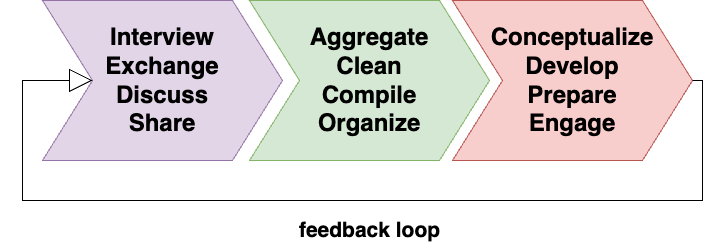
\includegraphics[width=1\linewidth]{Modele_Latex_CNRIUT2025//images/Diagrams-Simplified framework chain Our approach.drawio.png}
    \caption{Chaîne d'approche simplifiée}
    \label{fig:approach-simplified}
\end{figure}

La première phase (en violet) de discussion est primordiale et, peut-être, la plus longue et la plus importante étape dans notre cadre. Pour que le système soit fiable, efficace et accepté, vous devez faire sentir à tous les acteurs impliqués qu'ils sont écoutés et qu'ils sont intéressés par le système. En prouvant que c'est un outil vital pour eux et l'alliance et que suivre un tel cadre est important pour le bien-être de l'alliance et de toutes les actions (y compris les leurs).

La deuxième phase (en vert) évalue les résultats de la première étape. Comment pouvons-nous agglomérer et compiler les informations de la première phase pour qu'elles soient à la fois logiques et pertinentes pour tous ? C'est ici que les experts et les chefs de projet devront discuter et échanger sur la meilleure façon de compiler toutes les données acquises à partir de la phase 1 pour développer la solution.

Enfin, la troisième phase, en rouge, est la conception, le développement et la construction du système de suivi et d'évaluation concret. Représenté comme un entrepôt de données pour l'impact et une plateforme de partage de connaissances et de collaboration opérée à travers les technologies sémantiques et les technologies du web sémantique.

Chaque étape inclut des plans pour évaluer le changement à l'intérieur de l'université et de l'alliance dans son ensemble. À travers la planification informative et les actions de suivi pour gérer la résistance et simplement guider le changement à travers l'alliance, pour qu'il soit perçu positivement. Il est clair, à partir de la revue de la littérature, que pour avoir un changement efficace, nous devons créer une boucle de rétroaction positive pour nous assurer que tous les acteurs impliqués dans l'action se sentent écoutés et entendus. 

\section{Résultats}
Pour cette première année, nous avons établi une méthodologie pour récupérer les indicateurs et besoins de chaque tâche dans l'alliance UNITA. De ces interviews utilisant cette méthodologie orientée impact, nous avons pu récupérer une liste conséquente d'informations. Informations que nous avons validé avec chaque tâche, puis avec l'équipe de l'observatoire d'impact de l'alliance européenne UNITA (tâche) 5.4. Enfin, après un premier nettoyage des données, elles furent utilisées au sein du data warehouse de UNITA en tant que meta-data. Les choix et discussions n'étant pas encore finalisés, nous n'avons pas encore de résultat sur les indicateurs d'impact (plus difficiles à demander et récolter). 
\begin{table}[h]
  \caption{Résultat des premières interviews}
  \begin{center}
    \begin{tabular}{|l|l|l|l|} \hline
    \textbf{Type d'indicateurs} & \textbf{Nombre d'indicateurs} \\ \hline
    Outputs & 160 \\ \hline
    Outcomes & 75 \\ \hline
    \end{tabular}
  \end{center}
\end{table}

\section{Remerciements}
Je souhaiterais remercier l'alliance UNITA pour son aide sur ce travail ainsi que sa participation comme modèle de base pour explorer ses possibilités et permettre d'améliorer les alliances universitaires de demain.

\printbibliography


\end{document}

